
\documentclass[11pt]{article}

% Packages
\usepackage{amsmath}
\usepackage{amssymb}
\usepackage{siunitx}
\usepackage{tikz}
\usetikzlibrary{arrows.meta,calc}

% Document information
\title{Actuator Force Requirements for Rail Control System}
\author{Jamison McCulloch-Cop, Reviewed By Darcy Ryan}
\date{\today}

\begin{document}

\maketitle

%------------------------------------------------
\section{System Definition}
%------------------------------------------------

Define the following parameters:

\begin{align*}
    L_1 &= \text{Length of beam} \\
    L_2 &= \text{Length of attached object} \\
    m_1 &= \text{Mass of beam} \\
    m_2 &= \text{Mass of attached object} \\
    r_f &= \text{Actuator attachment distance from pivot} \\
    \Delta\theta &= \text{Required angular displacement} \\
    t &= \text{Desired motion time} \\
    g &= \text{Gravitational acceleration}\\
    \Delta z &= \text{Linear distance} \\
    \dot{z} &= \text{Linear speed} \\
\end{align*}
The beam rotates about the left-hand pivot.



%------------------------------------------------
\section{Free Body Diagram}
%------------------------------------------------

\begin{center}
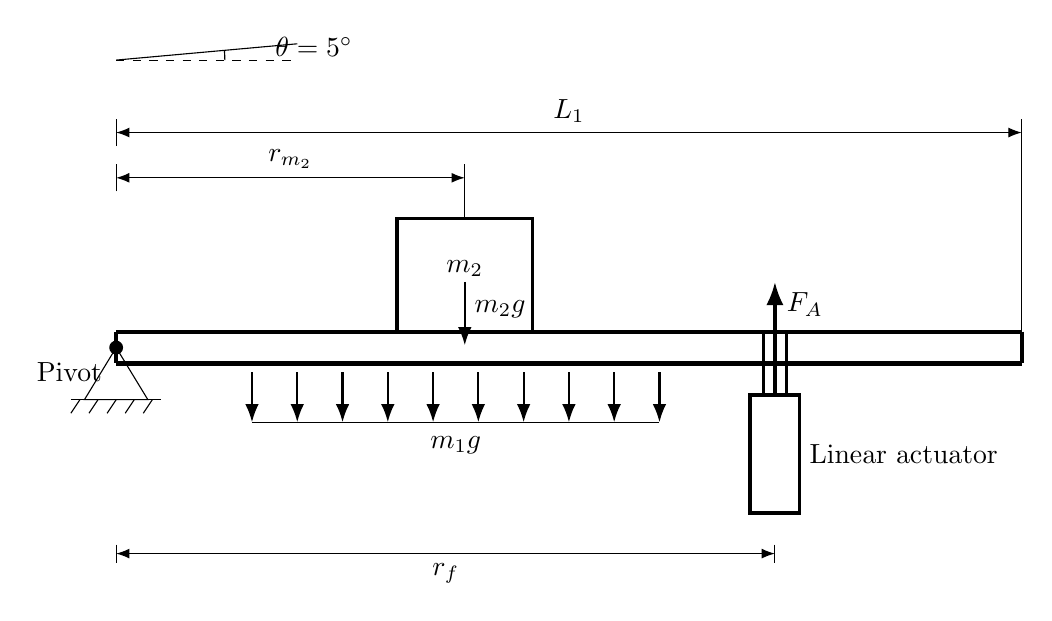
\begin{tikzpicture}[
    scale=1.15,
    >=Latex
]

%------------------------------------------------
% Beam
%------------------------------------------------

\draw[line width=1.5pt]
    (0,0) -- (10,0);

\draw[line width=1.5pt]
    (0,-0.35) -- (10,-0.35);

\draw[line width=1.5pt]
    (0,0) -- (0,-0.35);

\draw[line width=1.5pt]
    (10,0) -- (10,-0.35);

%------------------------------------------------
% Pivot
%------------------------------------------------

\filldraw (0,-0.175) circle (0.07);

\draw
    (0,-0.175) -- (-0.35,-0.75) -- (0.35,-0.75) -- cycle;

\draw
    (-0.5,-0.75) -- (0.5,-0.75);

\draw
    (-0.4,-0.75) -- (-0.5,-0.9);

\draw
    (-0.2,-0.75) -- (-0.3,-0.9);

\draw
    (0,-0.75) -- (-0.1,-0.9);

\draw
    (0.2,-0.75) -- (0.1,-0.9);

\draw
    (0.4,-0.75) -- (0.3,-0.9);

\node[left] at (-0.05,-0.45) {Pivot};

%------------------------------------------------
% Attached mass m_2
%------------------------------------------------

\draw[line width=1.2pt]
    (3.1,0) rectangle (4.6,1.25);

\node at (3.85,0.7) {$m_2$};

% Weight of attached mass
\draw[->,thick]
    (3.85,0.55) -- (3.85,-0.15);

\node[right] at (3.85,0.25) {$m_2g$};

%------------------------------------------------
% Distributed beam weight
%------------------------------------------------

\foreach \x in {1.5,2.0,2.5,3.0,3.5,4.0,4.5,5.0,5.5,6.0}
{
    \draw[->,thick]
        (\x, -0.45) -- (\x,-1.0);
}

\draw
    (1.5,-1.0) -- (6.0,-1.0);

\node at (3.75,-1.25) {$m_1g$};

%------------------------------------------------
% Actuator
%------------------------------------------------

% Actuator body
\draw[line width=1.2pt]
    (7.0,-2.0) rectangle (7.55,-0.7);

% Actuator rod
\draw[line width=1.2pt]
    (7.15,-0.7) rectangle (7.4,0);

% Actuator force
\draw[->,very thick]
    (7.275,-0.7) -- (7.275,0.55);

\node[right] at (7.3,0.3) {$F_A$};

\node[right] at (7.55,-1.35) {Linear actuator};

%------------------------------------------------
% Dimension: r_f
%------------------------------------------------

\draw[<->]
    (0,-2.45) -- (7.275,-2.45);

\draw
    (0,-2.35) -- (0,-2.55);

\draw
    (7.275,-2.35) -- (7.275,-2.55);

\node[below] at (3.64,-2.45) {$r_f$};

%------------------------------------------------
% Dimension: r_{m_2}
%------------------------------------------------

\draw[<->]
    (0,1.7) -- (3.85,1.7);

\draw
    (0,1.55) -- (0,1.85);

\draw
    (3.85,1.25) -- (3.85,1.85);

\node[above] at (1.925,1.7) {$r_{m_2}$};

%------------------------------------------------
% Dimension: L_1
%------------------------------------------------

\draw[<->]
    (0,2.2) -- (10,2.2);

\draw
    (0,2.05) -- (0,2.35);

\draw
    (10,0) -- (10,2.35);

\node[above] at (5,2.2) {$L_1$};

%------------------------------------------------
% Angle
%------------------------------------------------

\draw[dashed]
    (0,3.0) -- (2.0,3.0);

\draw
    (0,3.0) -- (2.0,3.18);

\draw
    (1.2,3.0) arc (0:5:1.2);

\node[right] at (1.65,3.15) {$\theta = 5^\circ$};

\end{tikzpicture}
\end{center}

where

\begin{align*}
    r_{m_1} &= \text{Distance from pivot to beam center of mass} \\
    r_{m_2} &= \text{Distance from pivot to object center of mass}
\end{align*}


%------------------------------------------------
\section{Gravitational Torque}
%------------------------------------------------

The torque due to gravity is
\[
    \tau_g = m_1 g r_{m_1}\cos\theta
           + m_2 g r_{m_2}\cos\theta
\]

The maximum gravitational torque occurs at
\[
    \theta = 0
\]

giving
\[
    \tau_{g,\max}
    = m_1 g r_{m_1} + m_2 g r_{m_2}
\]

%------------------------------------------------
\section{Angular Acceleration}
%------------------------------------------------

Assume a symmetric motion profile where the beam starts and
ends at rest, accelerating for the first half of the motion
and decelerating for the second half.

The angular displacement is
\[
    \Delta\theta = \frac{\alpha t^2}{4}
\]

Thus,
\[
    \boxed{
        \alpha = \frac{4\Delta\theta}{t^2}
    }
\]

%------------------------------------------------
\section{Rotational Inertia}
%------------------------------------------------

The beam inertia about the rail pivot (uniform rod, pivot at one end) is
\[
    I_1 = \frac{1}{3}m_1 L_1^2
\]

The payload must be taken about the \emph{same} pivot. If the payload centre of mass
lies a distance $r_{m_2}$ from the pivot, the parallel-axis contribution is
\[
    I_2 = I_{2,\mathrm{cm}} + m_2 r_{m_2}^2.
\]
For a compact aircraft, $I_{2,\mathrm{cm}}$ is often small compared with $m_2 r_{m_2}^2$, so
\[
    I_2 \approx m_2 r_{m_2}^2
\]
is a useful lower-bound model. Using only $\frac{1}{3}m_2 L_2^2$ about the payload's own
end (and omitting $m_2 r_{m_2}^2$) understates inertia when the aircraft sits far out on the rail.

Therefore,
\[
    \boxed{
        I_T = I_1 + I_2
        = I_1 + I_{2,\mathrm{cm}} + m_2 r_{m_2}^2
    }
\]

%------------------------------------------------
\section{Acceleration Torque}
%------------------------------------------------

The torque required to accelerate the rotating system is
\[
    \tau_a = I_T \alpha
\]

Substituting the angular acceleration,
\[
    \boxed{
        \tau_a = I_T
        \left( \frac{4\Delta\theta}{t^2} \right)
    }
\]

%------------------------------------------------
\section{Total Required Torque}
%------------------------------------------------

The maximum torque requirement occurs at the beginning of
motion where gravity torque is largest and angular
acceleration is applied.

\[
    \tau_T = \tau_{g,\max} + \tau_a
\]

Substituting previous expressions,
\[
    \boxed{
        \tau_T =
        m_1 g r_{m_1}
        + m_2 g r_{m_2}
        + I_T \left( \frac{4\Delta\theta}{t^2} \right)
    }
\]

%------------------------------------------------
\section{Actuator Force}
%------------------------------------------------

If the actuator force acts perpendicular to the beam at a
distance $r_f$ from the pivot,
\[
    \tau_A = F_A r_f
\]

Therefore,
\[
    \boxed{
        F_A = \frac{\tau_T}{r_f}
    }
\]

Substituting for total torque,
\[
    \boxed{
        F_A =
        \frac{
            m_1 g r_{m_1}
            + m_2 g r_{m_2}
            + I_T \left( \frac{4\Delta\theta}{t^2} \right)
        }{r_f}
    }
\]

More generally, if the actuator force is not perpendicular
to the beam,
\[
    \tau_A = F_A r_f \sin\phi
\]

and
\[
    \boxed{
        F_A = \frac{\tau_T}{r_f\sin\phi}
    }
\]

where $\phi$ is the angle between the actuator force vector
and the beam.

%------------------------------------------------
\section{Linear Distance and Speed}
%------------------------------------------------

For a vertical actuator mounted beneath the attachment
point, the vertical displacement of the attachment point is
\[
    \boxed{
        \Delta z = r_f \sin(\Delta\theta)
    }
\]

The corresponding average linear speed is
\[
    \boxed{
        \dot z = \frac{\Delta z}{t}
    }
\]

It is important to note that $\Delta z$ represents the
vertical motion of the attachment point. The true actuator
stroke should be determined from the actuator mounting
geometry and may differ from this value if the actuator
does not remain vertical throughout the motion.

%------------------------------------------------
\section{Safety Factor}
%------------------------------------------------

Including a design safety factor $N_s$,
\[
    \boxed{
        F_{\mathrm{design}} = N_s F_A
    }
\]

where typically
\[
    N_s = 1.5\text{--}3
\]
depending on the application.

%------------------------------------------------
\section{Ball Screw Motor Requirements}
%------------------------------------------------

Let
\begin{align*}
    F_A &= \text{Required actuator force} \\
    L_s &= \text{Ball screw lead (linear travel per revolution)} \\
    \eta &= \text{Ball screw efficiency} \\
    T_m &= \text{Required motor torque} \\
    n   &= \text{Required motor rotational speed}
\end{align*}

The ball screw converts motor rotation into linear motion. The
required motor torque is

\[
    \boxed{
        T_m = \frac{F_A L_s}{2\pi\eta}
    }
\]

where
\begin{itemize}
    \item $F_A$ is the actuator force,
    \item $L_s$ is the ball screw lead,
    \item $\eta$ is the mechanical efficiency of the ball screw.
\end{itemize}

The required motor speed is obtained from the actuator linear speed:

\[
    \boxed{
        n = \frac{\dot{z}}{L_s}
    }
\]

where $n$ is expressed in revolutions per second.

Converting to revolutions per minute (RPM),

\[
    \boxed{
        n_{\mathrm{RPM}} = 60\left(\frac{\dot{z}}{L_s}\right)
    }
\]

The mechanical power required from the motor is

\[
    \boxed{
        P_m = T_m\omega
    }
\]

where

\[
    \omega = 2\pi n
\]

is the motor angular velocity.

Equivalently,

\[
    \boxed{
        P_m = \frac{F_A\dot{z}}{\eta}
    }
\]

which provides a useful verification of the motor sizing calculations.


%------------------------------------------------
\section{Notes on Implementation}
%------------------------------------------------

\begin{itemize}
    \item Use a consistent definition of $\theta$ (e.g.\ $\theta=0$ horizontal) when evaluating $\tau_g$.
    \item For a triangular velocity profile, peak linear speed is about twice the average $\dot{z}=\Delta z/t$; size motor RPM from the peak unless a softer profile is specified.
    \item Prototype masses ($\sim 5\,\mathrm{kg}$ stand-in) and full-size Fighter mass ($<7\,\mathrm{kg}$ MTOW) must not be mixed with outdated placeholders (e.g.\ $11\,\mathrm{kg}$).
    \item $r_{m_2}$ is the distance from the \emph{rail pivot} to the payload centre of mass, not $L_2/2$ unless the payload is actually centred that close to the pivot.
\end{itemize}

\end{document}
